\documentclass[12pt]{article}

\usepackage{amsmath}
\usepackage{amssymb}
\usepackage[linesnumbered,ruled,vlined]{algorithm2e}
\usepackage{verbatim}
% To allow footnotes inside tables: (https://tex.stackexchange.com/questions/109467/footnote-in-tabular-environment)
\usepackage{footnote}
\makesavenoteenv{tabular}
\usepackage{graphicx}
\graphicspath{ { images/ } }

\DeclareMathOperator*{\argmax}{arg\,max}

\title{CS 188: Artificial Intelligence}
\author{Matthew Signorotti}
\date{Spring 2020}

\begin{document}

\maketitle

\tableofcontents

\section{Agents}

In artificial intelligence, we control an \textbf{agent} which has goals or preferences and performs actions in an environment. A \textbf{reflex agent} doesn't think about the consequences of its actions and acts solely based on the state of the world. \textbf{Planning agents}, like humans, simulate possible courses of action and choose the best one.

\section{Search}

In a search problem, we have a \textbf{state space}, \textbf{successor function}, \textbf{start state}, and \textbf{goal test}. In AI, the successor function typically maps from states and actions to costs and successor states. Often, the state space is too large to construct in memory; rather we construct it on demand in graph or tree form.

Many different approaches in search reduce to the \textbf{tree search} algorithm, only with a specific policy for queueing states (fringe). \textbf{Graph search} is essentially the same, but with the added optimization that we can only add a state's children to the fringe once.
\begin{algorithm}[h]
\caption{Tree search}

\SetKwInput{Input}{Input}
\SetKwFunction{TreeSearch}{TreeSearch}
\SetKwInput{Output}{Output}
\SetKwProg{Fn}{Function}{:}{}
\SetKwFunction{FringeOfType}{FringeOfType}
\SetKwFunction{Pop}{Pop}

\Fn{\TreeSearch{graph, start, destination, fringetype}}{
	\Input{graph, start state, destination state, fringetype}
	\Output{a path from start to finish, or failure}
	\BlankLine
	
	fringe $\gets$ \FringeOfType{fringetype}\;
	add starting state to fringe\;
	\While{fringe is not empty}{
		state $\gets$ \Pop{fringe}\;
		\lIf{state is destination}{\KwRet{state}}
		add state's children to fringe\;
	}
	\KwRet{failure}\;
}
\end{algorithm}

A search strategy can be \textbf{complete} --- guaranteed to find a solution to a search problem --- or \textbf{optimal} --- guaranteed to find a lowest-cost path to a goal state. Below are several \textbf{uninformed search strategies} specifically for the tree search algorithm. Note that for a given problem, a search algorithm has a branching factor $b$, the greatest possible increase in nodes on the fringe per dequeued node; $m$, the maximum depth; and $s < m$, the shallowest solution depth.
\begin{center}
\begin{tabular}{ |c|c|c|c|c|c| } 
\hline
Search strategy & Complete? & Optimal? & Time & Space \\
\hline
Depth-first search & No & No & $O(b^m)$ & $O(bm)$ \\
Breadth-first search & Yes & No & $O(b^s)$ & $O(b^s)$ \\
Uniform cost search & Yes & Yes & $O(b^{C^*/\epsilon})$\footnote{$C^*$ is the optimal path cost; $\epsilon$ is the minimal cost between two states.} & $O(b^{C^*/\epsilon})$ \\
\hline
\end{tabular}
\end{center}

Unlike uninformed search strategies, \textbf{informed search strategies} employ some notion of ``closeness'' to the goal. Concretely, this notion may be provided by a heuristic, a function from states to estimate values. Here are the properties of additional tree and graph search strategies.
\begin{center}
\begin{tabular}{ |c|c|c|c|c|c| } 
\hline
Search strategy & Complete? & Optimal? \\
\hline
Greedy (tree) search & No & No \\
A* (tree) search & Yes\footnotemark & Yes\footnotemark[\value{footnote}]\footnotetext{Complete and optimal under an \textbf{admissible} heuristic: $\forall s (0 \leq h(s) \leq h^*(s))$} \\
A* (graph) search & Yes\footnotemark & Yes\footnotemark[\value{footnote}]\footnotetext{Complete and optimal under an admissible and \textbf{consistent} heuristic: intuitively, for all transitions from $s_1$ to $s_2$, $h(s_1) - h(s_2) \leq cost(s_1, s_2)$} \\
\hline
\end{tabular}
\end{center}
Admissible heuristics can be compared through dominance. $h_a$ is said to dominate $h_b$ if $\forall s (h_a(s) \geq h_b(s))$. Generally, the higher the heuristic the better; for example the max of admissible (consistent) heuristics is also admissible (consistent) but leads to better performance.

\section{Constraint satisfaction problems (CSPs)}

CSPs are \textbf{identification problems}: we must identify a solution and unlike search, how we arrive at a solution does not matter. CSPs consist of variables, a domain for the variables, and constraints, which restrict the set of allowed variable combinations. In general, CSPs are NP-hard. They can be solved in a reasonable amount of time, for instance by solving a search problem whose state space is partial assignments of variables. \textbf{Backtracking search} is a generalized algorithm for CSPs, similar to depth-first search. Under assumptions that we can select values and variables and check consistency in constant time, the runtime is $O(d^n)$, with $n$ the number of variables and $d$ the number of values for a variable.

\begin{algorithm}[h]
\caption{Backtracking search}
\SetKwInput{Input}{Input}
\SetKwInput{Output}{Output}

% Just playing around with the package:
% \SetKw{Kw}{thetext}
% \SetKwFunction{SelectUnassigned}{SelectUnassignedVariable}
% \SelectUnassigned\;
% \Kw{test}\;

\SetKwProg{Fn}{Function}{:}{}
\SetKwFunction{Backtracking}{Backtracking}
\SetKwFunction{Unassigned}{SelectUnassignedVariable}
\SetKw{in}{in}
\SetKwFunction{Order}{OrderDomainValues}

\Fn{\Backtracking{assignment}}{
	\Input{an assignment of variables (empty by default)}
	\Output{the completed assignment of variables, or failure}
	\BlankLine
	
	\lIf{assignment is complete}{\KwRet{assignment}}
	var $\gets$ \Unassigned{variables, assignment}\;
	\ForEach{value \in{\Order{var, assignment}}}{
		\If{value consistent with assignment given constraints}{
			let var $\gets$ value in the assignment\;
			\tcc{Invariant: if input was consistent, assignment is still consistent}
			result $\gets$ \Backtracking{assignment}\;
			\lIf{result is not failure}{\KwRet{result}}
			remove var from assignment\;
		}
	}
	\KwRet{failure}\;
}
\end{algorithm}

\subsection{Filtering}

In \textbf{filtering}, we check the domains of unassigned variables ahead of time by removing values we know will result in backtracking. In the naive technique of \textbf{forward checking}, whenever a value is assigned to a variable, the domains of all unassigned variables sharing constraints with that variable are pruned.

This technique generalizes into the idea of \textbf{arc consistency}, which is typically implemented with the AC-3 algorithm (runtime of $O(ed^3)$, with $e$ the number of arcs and $d$ the size of the largest domain). In arc consistency, we have a directed constraint graph in which $a \to b$ means that $a$ shares a binary constraint with $b$ (the graph has no higher-order constraints). We say there is arc consistency, i.e. the arcs are consistent, if for all edges $a \to b$, all possible values of $a$ have a value of $b$ for which the combination of $a$ and $b$ is consistent.
\begin{algorithm}[h]
\caption{AC-3}

\SetKwInput{Input}{Input}
\SetKwInput{Output}{Output}
\SetKwProg{Fn}{Function}{:}{}
\SetKwFunction{AC}{AC-3}
\SetKw{in}{in}
\SetKwFunction{Pop}{RemoveFirst}
\SetKwFunction{RemoveInconsistent}{RemoveInconsistentValues}
\SetKwFunction{Neighbors}{Neighbors}
\SetKwFunction{Domain}{Domain}

\Fn{\AC{csp}}{
	\Input{csp, a CSP with a binary directed constraint graph}
	\Output{the CSP, with arc consistency and possibly reduced variable domains}
	\BlankLine
	
	initialize empty queue\;
	\lForEach{edge $(X_i, X_j)$ \in{csp}}{enqueue $(X_i, X_j)$}
	\While{queue is not empty}{
		$X_i, X_j \gets$ \Pop{queue}\;
		\If{\RemoveInconsistent{$X_i, X_j$}}{
			\ForEach{$X_k$ \in{\Neighbors{$X_i$}}}{
				enqueue $(X_k, X_i)$ if not enqueued already\;
			}
		}
	}
	\KwRet{csp}\;
}

\Fn{\RemoveInconsistent{$X_i, X_j$}}{
	removed $\gets$ false\;
	\ForEach{$x_i$ \in{\Domain{$X_i$}}}{
		\If{no $x_j$ \in \Domain{$X_j$} satisfies binary constraint(s) between $X_i$ and $X_j$}{
			delete $x_i$ from \Domain{$X_i$}\;
			removed $\gets$ true\;
		}
	}
	\KwRet{removed}\;
}
\end{algorithm}

The idea of $k$-consistency generalizes arc consistency (which is really $2$-consistency). In \textbf{$\mathbf{k}$-consistency}, for any subset of $k$ variables, any consistent assignment of $k - 1$ variables guarantees at least one consistent value for the $k$th variable. In \textbf{strong $\mathbf{k}$-consistency}, any subset of $k$ variables is $k$-, $(k - 1)$-, $\ldots$, $1$-consistent, and we can be assured there will be no backtracking.

\subsection{Ordering}

Rather than fixing an ordering of variables and values, we can also heuristically compute the next variable or value on the fly. The principle of \textbf{minimum remaining values} says to select the variable which has the fewest valid remaining values in its domain. The principle of \textbf{least constraining value} says to select the value which prunes the fewest values from the remaining unassigned variables.

\subsection{Structure}

By exploiting special problem structure, we can achieve better runtime.
\begin{itemize}
\item If the constraint graph contains $n$ variables but can be broken into independent sub-graphs of $c$ variables, we can solve the CSP in $O\left((n/c) (d^c)\right)$ time.
\item If the graph is connected and contains no loops (is \textbf{tree-structured}), we can solve in $O\left(nd^2\right)$ time. First choose an arbitrary variable as the root vertex and direct all edges so as to form a directed acyclic graph. Next, perform a forward arc consistency pass along a topological sort, from sink to root, and finally perform an forward assignment from root to sink, arbitrarily choosing a value for each variable which works with the variable's parents' values. The forward assignment will succeed if no domain is empty.
\item We can select a \textbf{cutset} of vertices, without which the constraint graph would be acyclic. Then, condition on values for this cutset, pruning for each assignment the domains of unassigned variables. For a cutset of size $c$, we get a runtime of $O\left((d^c)(n - c)d^2\right)$.
\item We can decompose a CSP with a cyclic constraint graph to an acyclic problem of \textbf{mega-variables}.
\end{itemize}

\subsection{Local search}

Aside from backtracking, we can also start with a random, likely inconsistent assignment and iteratively improve on it, hopefully converging to a satisfying assignment. This is the simple idea of \textbf{local search}. While the current assignment is inconsistent, we can select a variable arbitrarily and select and assign a value according to the \textbf{min-conflicts heuristic}, which chooses the value resulting in the fewest conflicts. In randomly generated CSPs, this method appears to perform roughly linearly in time, except around a certain problematic ratio of constraints to variables.

\subsection{Optimization}

We can formulate these problems as optimization problems, for instance minimizing the number of constraints violated. These are numerous algorithms available.
\begin{itemize}
\item \textbf{Hill climbing}: Start wherever, move to the best neighboring state until no neighbors are better than the current state.
\begin{itemize}
\item Can also employ \textbf{beam search}, in which we track the $k$ best states at each time step.
\end{itemize}
\item \textbf{Simulated annealing}: Takes a schedule for a temperature parameter. Until the temperature parameter becomes $0$, it selects the current temperature parameter and randomly selects a successor. If the successor is better than the current state, it switches the state; otherwise it selects according to probability $e^{\Delta E/T}$ where $\Delta E$ ($\leq 0$) is the change in values from the current to successor states.
\item \textbf{Genetic algorithms}: Use a natural selection metaphor, maintaining a population of $N$ individuals in each generation. Incorporates pairing/mating, crossover, and mutation operators.
\end{itemize}

\section{Games}

\textbf{Games}, otherwise known as \textbf{adversarial search problems}, are scenarios in which the agent has an adversary actively working in ways which may keep the agent from its goal. Games may or may not have deterministic or stochastic outcomes, have a variable number of players, and be \textbf{zero-sum} (in terms of utilities or winnings), or make perfect information available to the agent.

\subsection{Minimax}

In the \textbf{minimax} algorithm, we assume that the opposing player plays optimally. We start with a game tree whose vertices are game states and whose leaves are terminal game states whose values, the winnings for our agent, reflect some property of the game. In each game state, a certain player is next to move. Depending on the player (our agent or an adversary), the state should be assigned a value which is the maximum or minimum of the children vertices.

Due to runtime issues, it is often infeasible to construct this entire tree. In \textbf{depth-limited minimax}, we can instead limit the depth of the search tree and use an \textbf{evaluation function} to treat non-leaf vertices at the terminal depth as leaves. We can also employ the previous technique of iterative deepening to combine the benefits of DFS and BFS.

\subsubsection{Alpha-beta pruning}

We can improve the performance of minimax with \textbf{alpha-beta pruning}. While recursively computing the children's values, we track two additional values, $\alpha$ and $\beta$. At any time, we ensure that $\alpha$ is the maximum child value seen by a maximizing vertex on the path from this vertex to the root, while $\beta$ is the minimum child value seen by a minimizing vertex on the path from this vertex to the root. We can stop examining (``prune'') the sub-trees of children of the current vertex when we're certain this vertex value will be at least $\beta$ (for maximization vertices) or at most $\alpha$ (for minimization vertices). Note that values for ``intermediate'' vertices may not be exact.

\subsection{Expectimax}

\textbf{Expectimax} is the same as minimax, except that instead of minimization vertices, we have expectation vertices. We assign a probability distribution over the values of these vertices' children and take the expected value of this distribution. Alpha-beta pruning is no longer feasible, unless we have bounds on vertex values.

\subsubsection{Mixed layer types}

Depending on the nature of the problem, we can have a combination of maximization, minimization, and expectation vertices in a game tree.

\subsection{General games}

So far, the game trees we have discussed have had one utility value at each vertex --- i.e. the games are zero-sum. However, the world may look different to different agents. One may want to assign different utilities for different agents at each vertex: at each node, each agent will only be concerned with their own utility.

\subsection{Utilities}

What exactly are these utilities we speak of? First, we establish the five \textbf{axioms of rationality}, which describe the existence of an agent's preference ordering over the set of outcomes:
\begin{enumerate}
\item \textit{Orderability}: $\forall A, B \left((A \succ B) \vee (B \succ A) \vee (A \sim B)\right)$
\item \textit{Transitivity}: $\forall A, B, C \left((A \succ B) \wedge (B \succ C) \implies (A \succ C)\right)$
\item \textit{Continuity}: $\forall A, B, C (A \succ B \succ C \implies \exists p \in [0, 1] ([p, A; 1 - p, C] \sim B))$, where $[p, A; 1 - p, C]$ is a lottery giving $A$ with probability $p$ or $C$ with probability $1 - p$
\item \textit{Substitutability}: $\forall A, B, C, p \in [0, 1] (A \sim B \implies [p, A; 1 - p, C] \sim [p, B; 1 - p, C])$
\item \textit{Monotonicity}: $\forall A, B, p \in [0, 1], q \in [0, 1] (A \succ B \implies (p \geq q \iff [p, A; 1 - p, B] \succ [q, A; 1 - q, B]))$
\end{enumerate}
If the above assumptions hold, there must exist a real-valued \textbf{utility function} $U$ such that
\begin{enumerate}
\item $\forall A, B (U(A) \geq U(B) \iff A \succeq B)$
\item $\forall L (U(L) \sim \sum_i p_i U(S_i))$, where $L$ is a lottery with probability $p_i$ for outcome $S_i$ (in the case of a discrete lottery)
\end{enumerate}
Naturally, this utility function is to be maximized. A valid utility function can yield another valid utility function under a positive linear transformation, i.e. $U_2(S) = aU_1(S) + b$ with $a > 0$. Hence, there are many utility functions for a given set of preferences which are \textbf{strategically equivalent}.

For outcomes which are numeric values, e.g. money, an agent can be \textbf{risk-averse}, preferring every lottery's expected value to the lottery itself; \textbf{risk-neutral}, being indifferent between the two; or \textbf{risk-seeking}, preferring every lottery to its expected value.

\section{Non-deterministic search}

In our previous game models, actions have led deterministically to certain intended game states. Now, we'd like to incorporate randomness into our models.

\subsection{Markov decision processes (MDPs)}

First we will develop the \textbf{Markov decision process} model. A Markov decision process consists of:
\begin{itemize}
\item A set of states $S$
\item A set of actions $A$
\item A start state
\item Possibly one or more terminal states
\item Possibly a \textbf{discount factor} $\gamma$
\item A \textbf{transition function} $T : S \times A \times S \to [0, 1]$, which for any $s$ and $a$ is a probability distribution over resulting states $s'$
\item A \textbf{reward function} $R : S \times A \times S \to \mathbb R$ specifying rewards/utilities of going from $s$ to $s'$ with action $a$
\end{itemize}
We can construct a game tree of states and \textbf{q-states}, which are chance nodes corresponding to both a state and action. We also define the utility function for a series of states $\{s_i\}$ and actions $\{a_i\}$ so that
\[ U(\left[s_0, a_0, s_1, a_1, s_2, \ldots\right]) = R(s_0, a_0, s_1) + R(s_1, a_1, s_2) + \cdots. \]
Note that this sum may be infinite, so we introduce either a \textbf{finite horizon} or a discount factor. With the former, we determine a set number of time steps as the lifespan of all agents, and after which the game simply ends. With finitely many time steps, the above sum is sure to be finite. And with a discount factor, replace the sum $R(s_0, a_0, s_1) + \cdots$ with $\sum_{i = 0}^\infty \gamma^i R(s_i, a_i, s_{i + 1})$. When $|\gamma| < 1$, the infinite sum is guaranteed to converge, much like a geometric series.

\subsubsection{The Bellman equation}

Solving MDPs amounts to finding a policy $\pi^* : S \to A$ determining an action to take from each state, in such a way that maximizes expected utility. (We don't just plan the sequence of states and actions due to the nondeterminism of the system. Also, reducing the space of solutions to functions $S \to A$ reduces the problem complexity.)

The \textbf{Bellman equation} is a condition for optimality. In general, it is a necessary condition, and it is sufficient in the context of MDPs. It defines the following:
\[ V^*(s) = \max_a \sum_{s'} T(s, a, s') \left[ R(s, a, s') + \gamma V^*(s') \right] \]
Or, more simply:
\begin{gather*}
Q^*(s, a) = \sum_{s'} T(s, a, s') \left[ R(s, a, s') + \gamma V^*(s') \right] \\
V^*(s) = \max_a Q^*(s, a)
\end{gather*}

\subsubsection{Value iteration}

\textbf{Value iteration} is one algorithm to converge to values which satisfy the Bellman equation.
\begin{algorithm}[h]
\caption{Value iteration}

\SetKwProg{Fn}{Function}{:}{}
\SetKwFunction{ValueIteration}{ValueIteration}
\SetKwInput{Output}{Output}

\Fn{\ValueIteration{}}{
	\Output{the value assignment $V^*$}
	\BlankLine
	
	\lForEach{state $s$}{$V_0(s) \gets 0$}
	$k \gets 0$\;
	\While{not converged}{
		\ForEach{state $s$}{$V_{k + 1}(s) \gets \max_a \sum_{s'} T(s, a, s') \left[ R(s, a, s') + \gamma V_k(s') \right]$\;}
		increment $k$;
	}
	\KwRet{$V_k$}\;
}
\end{algorithm}
Once the algorithm converges and outputs $V^*$, we can easily determine $Q^*(s, a)$ and then perform \textbf{policy extraction} to determine $\pi^*(s) = \operatorname{argmax}_a Q^*(s, a)$.

\subsubsection{Policy iteration}

Value iteration can be quite slow, at $O(|S|^2|A|)$. Since the policy from policy extraction typically converges faster than the values $V^*$, the \textbf{policy iteration} algorithm can yield significant performance gains.
\begin{algorithm}[h]
\caption{Policy iteration}

\SetKwInput{Output}{Output}
\SetKwProg{Fn}{Function}{:}{}
\SetKwFunction{PolicyIteration}{PolicyIteration}
\SetKwFunction{PolicyEvaluation}{PolicyEvaluation}
\SetKwFunction{PolicyImprovement}{PolicyImprovement}

\Fn{\PolicyIteration{}}{
	\Output{an optimal policy $\pi^*$}
	\BlankLine
	$i \gets 0$\;
	define an initial policy $\pi_0$\;
	\tcc{Initial policies which are close to optimal tend to converge faster}
	\While{policy is not converged}{
		$V^{\pi_i} \gets$ \PolicyEvaluation($\pi_i$)\;
		$\pi_{i + 1} \gets$ \PolicyImprovement($V^{\pi_i}$)\;
		increment $i$\;
	}
	\KwRet{$\pi_i$}\;
}
\end{algorithm}
\textbf{Policy improvement} is simply policy extraction on the values $V^{\pi_i}$ generated by policy evaluation. \textbf{Policy evaluation} entails solving the following system of equations:
\[ V^\pi(s) = \sum_{s'} T(s, \pi(s), s') \left[ R(s, \pi(s), s') + \gamma V^\pi(s') \right] \]
This can also be done by the following update rule, similar to that of value iteration, although this method is typically slower than simply solving the system of equations.
\[ V^\pi_{k + 1}(s) \gets \sum_{s'} T(s, \pi(s), s') \left[ R(s, \pi(s), s') + \gamma V^\pi_k(s') \right] \]

\subsection{Reinforcement learning}

Markov decision processes are an example of \textbf{offline planning}, in which agents have full knowledge of the transition and reward function. But perhaps the agent has no prior knowledge (\textbf{online planning}). It can perform exploration and receive feedback through the rewards it reaps. Using \textbf{reinforcement learning}, the agent can perform exploration and then \textbf{exploitation} to maximize expected utility under the model it constructs by interacting with the world.

There are two types of reinforcement learning: model-based and model-free.

\subsubsection{Model-based learning}

In \textbf{model-based learning}, we simply track the number of times we encounter each transition $(s, a, s')$ --- transitioning from $s$ to $s'$ through action $a$. By normalizing by the number of times we have been in state $s$ and chosen action $a$, we can develop a probability distribution $T(s, a, s')$ for each q-state $(s, a)$. This approach is remarkably effective, but maintaining counts for each transition $(s, a, s')$ can be costly.

\subsubsection{Model-free learning}

\textbf{Model-free learning} can be divided into two approaches. \textbf{Passive reinforcement learning} includes direct evaluation and temporal difference learning and typically involves estimating the values under a specific policy, without actively improving the policy itself. In \textbf{direct evaluation}, we fix a policy $\pi$ and simply evaluate the average reward transitioning out of each state under policy $\pi$. In \textbf{temporal difference learning}, at each time step we compute an estimate of $V^\pi(s)$, $sample = R(s, \pi(s), s') + \gamma V^\pi(s')$, and update according to an exponential moving average $V^\pi(s) \gets (1 - \alpha)V^\pi(s) + \alpha \cdot sample$, with the learning rate $\alpha \in [0, 1]$. Compared to direct evaluation, this method doesn't wait until the end to estimate $V^\pi$, gives less weight to older, less accurate samples, and converges to the true $V^\pi$ more quickly.

\textbf{Active reinforcement learning} techniques seek to use incoming information to actively improve the current policy. One could use temporal difference learning or direct evaluation in conjunction with model-based learning to estimate $T$ and $R$ and update a policy, but \textbf{Q-learning} avoids the need to use model-based learning. It follows these two update rules: $sample = R(s, a, s') + \gamma \max_{a'} Q(s', a')$ and $Q(s, a) \gets (1 - \alpha) Q(s, a) + \alpha \cdot sample$, where again $\alpha$ is a learning rate in $[0, 1]$. One potential downside is that we need to store a value for every q-value; this problem is avoided by \textbf{approximate Q-learning}, which computes state values and q-values according to
\begin{align*}
V(s) &= \sum_{i = 1}^n w_i f_i(s) \\
Q(s, a) &= \sum_{i = 1}^n w_i f_i(s, a).
\end{align*}
It does this by computing $difference = [R(s, a, s') + \gamma \max_{a'} Q(s', a')] - Q(s, a)$ and letting $w_i \gets w_i + \alpha \cdot difference \cdot f_i(s, a)$.

For Q-learning and approximate Q-learning, we want to strike a balance between exploration, to see which actions might work best, and exploitation, to reap the benefits of taking these actions. One option is the \textbf{$\epsilon$-greedy policy}, which explores randomly with probability $\epsilon$ and exploits the current best action with probability $1 - \epsilon$. Another option is using an \textbf{exploration function}, whereby we replace $\max_{a'} Q(s', a')$ in the Q-learning update with $\max_{a'} f(s', a')$. A common choice of exploration function in this case is $f(s, a) = Q(s, a) + k/N(s, a)$, with $N(s, a)$ being the number of times we have visited q-state $(s, a)$.

\section{Bayesian networks}

Due to memory issues, representing joint probability distributions by enumerating the probability of every outcome is problematic. For any joint distribution we can try computing a joint probability by processing all the variables one by one, conditioning for each variable on all the ancestors processed. However, this has the same problem!

A \textbf{Bayesian network} solves this problem through a simplifying assumption: that we can condition on only the direct parents of each variable in a directed acyclic graph. Specifically, the joint probability mass function (for a discrete joint distribution) is defined as
\begin{multline*}
P(X_1 = x_1, \ldots, X_n = x_n) \\
= \prod_{i = 1}^n P(X_i = x_i | X_{p(i)_1} = x_{p(i)_1}, \ldots, X_{p(i)_{|p(i)|}} = x_{p(i)_{|p(i)|}}),
\end{multline*}
where $p(i)$ is the indices of the direct parents of variable $i$.

Alternatively, a Bayesian network can be viewed as a joint distribution, again coupled with a directed acyclic graph, such that each variable is independent of each of its non-descendants when conditioned on its parents. These two definitions are equivalent.

\subsection{Inference}

In the context of Bayesian networks, \textbf{inference} is the task of computing some sub-distribution, such as a conditional distribution or a more specific joint distribution, for a Bayesian network.

\subsubsection{Enumeration}

One approach is to enumerate the entire joint probability table, pick the relevant rows, and compute the new distribution from there.

\subsubsection{Variable elimination}

A more efficient approach is to ``eliminate'' variables one by one. Specifically, this approach picks an elimination order $O$ which is a list of hidden variables to eliminate. We could always compute the sum
\[ \sum_{O_1, \ldots, O_{|O|}}\ \prod_{i = 1}^n P(X_i = x_i | X_{p(i)_1} = x_{p(i)_1}, \ldots, X_{p(i)_{|p(i)|}} = x_{p(i)_{|p(i)|}}), \]
as in enumeration, but elimination observes that we can exploit the distributive property to try moving the sum over each hidden variable $O_i$ as far as it can go inward, rearranging terms as necessary by commutativity. We do this for each variable $O_i$ in the order given by $O$. From the final table which contains no hidden variables, we can find the desired probability distribution.

Note that in this process, we don't need to normalize intermediate distributions --- we can hold out until the end. One of these intermediate, unnormalized probability distributions is referred to as a \textbf{factor}.

\subsection{Sampling}

Inference calculates exact distributions, but we can also estimate them through the \textbf{sampling} process. In \textbf{prior sampling}, we simulate the network by generating samples for each variable in the joint distribution in a variable order given by a topological sort of the Bayesian network's DAG. \textbf{Rejection sampling} is much the same except that we can immediately reject any sample inconsistent with the restricted ``evidence'' variables.

In \textbf{likelihood weighting}, we start by actually setting all evidence variables to their desired values, and then sample the rest of the variables in a topological sort order. We then weight each sample by multiplying by the probability of each evidence variable value given its parents' values.

\subsection{D-separation}

\textbf{D-separation} is an algorithm which allows us to conclude complex conditional independence relationships. First, we graphically define the canonical forms of active and inactive triples as follows:
\begin{center}
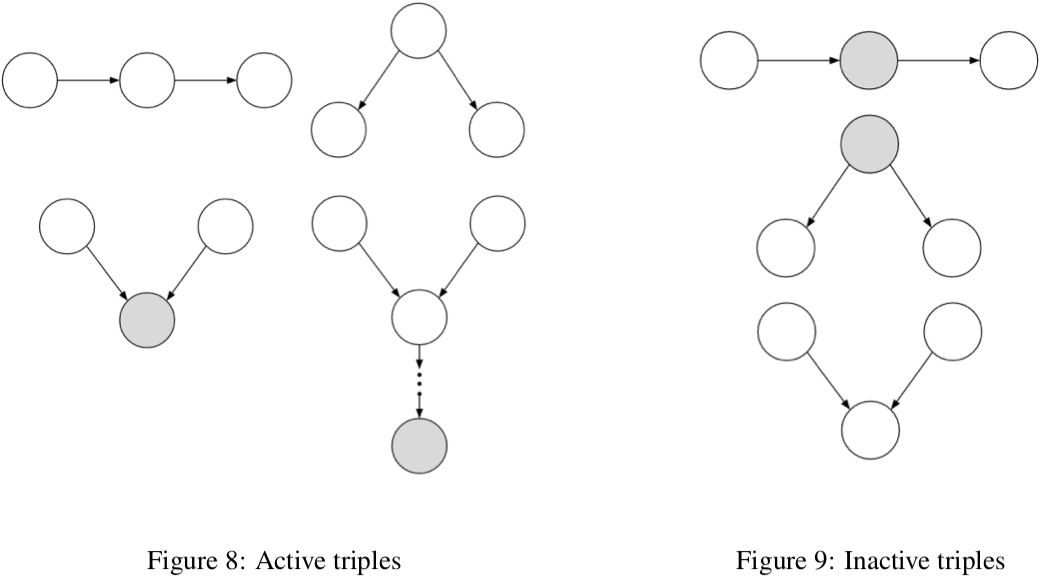
\includegraphics[width=.8\textwidth]{images/triple_graphs}
\end{center}
Above, shaded vertices are those variables which have known values, i.e. are being conditioned on.

Given two variables $X$ and $Y$, variables $\{Z_1, \ldots, Z_k\}$ being conditioned on, and an undirected path between the two (ignoring edge directions), we say that the path \textbf{d-connects} $X$ and $Y$ if, after decomposing the path into triples (segments of three vertices), all triples are active.

If not a single undirected path between $X$ and $Y$ d-connects $X$ and $Y$, then the d-separation algorithm concludes that $X$ and $Y$ are conditionally independent given $\{Z_1, \ldots, Z_k\}$.

\subsection{Markov models}

\textbf{Markov models} are Bayesian networks which are a single infinite chain index by time, and whose variables all share the same ``stationary'' conditional probability table.

The \textbf{mini-forward algorithm} marginalizes the variables in a Markov model, essentially by performing repeated matrix multiplication. Hence, we can solve for a \textbf{stationary distribution} of the Markov model's state by solving the appropriate matrix equation.

\subsection{Hidden Markov models}

In the same vein, \textbf{hidden Markov models} add a second set of evidence variables which are observed every time step and depend only on the true state variable at that time step. The \textbf{sensor model} is the CPT of the evidence given the true state, and this model is assumed to be stationary, like the state transition CPT.

The \textbf{belief distribution}, the distribution on the state at time $t$ given all evidence from times $1, \ldots, t$ is updated through the \textbf{forward algorithm}, which computes a matrix multiplication update step as before and then weights the output belief distribution according to the evidence observed.

\subsubsection{Viterbi algorithm}

The \textbf{Viterbi algorithm} solves for the most likely path from time steps $1, \ldots, t$ given evidence from time steps $1, \ldots, t$. Since the most likely path's probability is simply the transition probability from state $t - 1$ to state $t$, we can easily find this most likely path given the most likely paths and associated probabilities of all paths ending in each state at time $t - 1$ --- in other words, by using dynamic programming.
\begin{algorithm}[h]
\caption{Viterbi algorithm}

\SetKwInput{Output}{Output}
\SetKwProg{Fn}{Function}{:}{}
\SetKwFunction{Viterbi}{Viterbi}

\Fn{\Viterbi{}}{
	\Output{a most likely sequence of hidden states $x^*_{1:N}$}
	\BlankLine
	\tcc{Forward pass}
	\For{$t \gets 1, \ldots, N$}{
		\For{$x_t \in \mathcal X$}{
			\uIf{$t = 1$}{$m_t[x_t] \gets P(x_t) P(e_0 | x_t)$\;}
			\Else{
				$a_t[x_t] \gets \argmax_{x_{t - 1}} P(x_t | x_{t - 1}) m_{t - 1}[x_{t - 1}]$\;
				$m_t[x_t] \gets P(e_t | x_t) P(x_t | a_t[x_t]) m_{t - 1}[a_t[x_t]]$\;
			}
		}
	}
	$x^*_N \gets \argmax_{x_N} m_N[x_N]$\;
	\BlankLine
	\tcc{Backward pass}
	\For{$t \gets N, \ldots, 2$}{
		$x^*_{t - 1} \gets a_t[x^*_t]$\;
	}
	\KwRet{$x^*_{1:N}$}\;
}
\end{algorithm}

\subsubsection{Particle filtering}

\textbf{Particle filtering} is much like sampling, except that rather than sampling all the variables throughout time, we allow particles to ``filter'' through the graph. Particle filtering consists of a time elapse step, where we sample new values for each particle given the current value and the transition model. In the observation update step, we weight using the current observation, then normalize to create a new probability distribution, aggregate by particle value, and resample particles from this distribution. If normalization fails since all weighted probabilities are $0$, then we reinitialize new particles uniformly.

\section{Decision networks}

\textbf{Decision networks} are an extension of Bayesian networks and consist of \textbf{chance nodes} (as in Bayesian networks), \textbf{action nodes} (which we control), and \textbf{utility nodes} (which are children of chance and action nodes). These three nodes are represented by ovals, rectangles, and diamonds, respectively.

Expected utility can be maximized by observing evidence and using inference to calculate the posterior probabilities of unknown variables. Using this posterior distribution, calculate for each action the expected utility under that action and find the maximum.

We can unravel such a network into an \textbf{outcome tree}, where the root node corresponds to the action we choose, and children nodes are chance nodes leading to certain utility values with some probabilities.

\subsection{The value of perfect information}

We can compute the expected utility of knowing some additional variable with certainty minus the expected utility knowing only the standard evidence variables. This ``\textbf{value of perfect information}'' is nonnegative and generally non-additive for different possible additional evidence variables. It is also \textbf{order-independent}: observing multiple new evidence variables provides the same value of perfect information regardless of the observation order.

\section{Machine learning}

TODO

\subsection{Neural networks}

TODO

\end{document}
